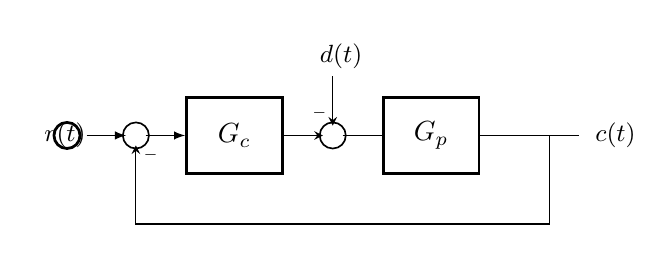
\begin{tikzpicture}
	% Paths, nodes and wires:
	\node[shape=rectangle, draw, line width=1pt, minimum width=1.215cm, minimum height=0.965cm] at (5.625, 8.75){} node[anchor=center, align=center, text width=0.827cm, inner sep=6pt] at (5.625, 8.75){$G_c$};
	\node[shape=rectangle, draw, line width=1pt, minimum width=1.215cm, minimum height=0.965cm] at (8.125, 8.75){} node[anchor=center, align=center, text width=0.827cm, inner sep=6pt] at (8.125, 8.75){$G_p$};
	\node[shape=circle, draw, line width=1pt, minimum width=-0.035cm] at (3.5, 8.75){};
	\draw[-latex] (4.5, 8.75) -- (5, 8.75);
	\node[shape=circle, draw, line width=0.6pt, minimum width=0.229cm] at (6.875, 8.75){};
	\draw[-stealth] (6.25, 8.75) -- (6.75, 8.75);
	\draw (7, 8.75) -- (7.5, 8.75);
	\node[shape=circle, draw, line width=0.6pt, minimum width=0.229cm] at (4.375, 8.75){};
	\draw[-stealth] (8.75, 8.75) -| (9.625, 7.625) |- (4.375, 7.625) -| (4.375, 8.625);
	\draw[-latex] (3.75, 8.75) -- (4.25, 8.75);
	\node[shape=rectangle, minimum width=0.715cm, minimum height=0.465cm] at (3.375, 8.75){} node[anchor=center, align=center, text width=0.327cm, inner sep=6pt] at (3.375, 8.75){\small $r(t)$};
	\node[shape=rectangle, minimum width=0.715cm, minimum height=0.465cm] at (10.375, 8.75){} node[anchor=center, align=center, text width=0.327cm, inner sep=6pt] at (10.375, 8.75){\small $c(t)$};
	\draw (9.625, 8.75) -- (10, 8.75);
	\node[shape=rectangle, minimum width=0.59cm, minimum height=0.215cm] at (4.563, 8.5){} node[anchor=center, align=center, text width=0.202cm, inner sep=6pt] at (4.563, 8.5){\tiny $-$};
	\node[shape=rectangle, minimum width=0.715cm, minimum height=0.465cm] at (6.875, 9.75){} node[anchor=center, align=center, text width=0.327cm, inner sep=6pt] at (6.875, 9.75){\small $d(t)$};
	\draw[-stealth] (6.875, 9.5) -- (6.875, 8.875);
    \node[shape=rectangle, minimum width=0.59cm, minimum height=0.215cm] at (6.706, 9.038){} node[anchor=center, align=center, text width=0.202cm, inner sep=6pt] at (6.706, 9.038){\tiny $-$};
\end{tikzpicture}